\begin{figure}[htbp]
			\centering
			\resizebox{\textwidth}{!}{%
				\begin{tikzpicture}[>=stealth, line width=0.8pt, font=\small,
					nodo/.style  = {circle, fill=white, draw=black,
						inner sep=0pt, minimum size=5pt, line width=0.8pt},
					cint/.style  = {circle, fill=white, draw=black,
						inner sep=0pt, minimum size=6pt, line width=0.9pt},
					LI/.style    = {line width=1.0pt, black},
					frecciaLI/.style = {->, >=stealth, line width=0.9pt, black},
					richiam/.style = {thin, gray, dashed},
					]
					
					%% ── Parametri geometrici globali ─────────────────────────────────────────
					\def\L{1.50}     % ell (cm)
					\def\tw{0.20}    \def\thA{0.34}  \def\thR{0.28}
					\def\sr{0.07}    \def\bw{0.14}   \def\gw{0.26}
					\def\DX{9.0}     % offset orizzontale tra pannelli (a) e (b)
					
					%% Posizioni nodi (origine = A di ciascun pannello)
					\pgfmathsetmacro{\xB}{\L}
					\pgfmathsetmacro{\xG}{0.5*\L}
					\pgfmathsetmacro{\xE}{1.5*\L}
					\pgfmathsetmacro{\xF}{3.5*\L}
					\pgfmathsetmacro{\xC}{4*\L}
					\pgfmathsetmacro{\xD}{5*\L}
					
					%% =========================================================================
					%% PANNELLO (a) — STRUTTURA CON CARICO MOBILE UNITARIO
					%% =========================================================================
					\begin{scope}[xshift=0cm, yshift=0cm]
						
						%% Posizione del carico mobile unitario
						\pgfmathsetmacro{\xP}{2.3*\L}
						
						%% ── Trave ────────────────────────────────────────────────────────────
						\draw[line width=2.2pt](0,0)--(\xD,0);
						
						%% ── Fibra inferiore ──────────────────────────────────────────────────
						\draw[line width=0.6pt, dashed, gray!55](0,-0.13)--(\xD,-0.13);
						
						%% ── Etichette nodi ───────────────────────────────────────────────────
						\node[above=0.04]at(0,0){$A$};
						\node[above=0.04]at(\xG,0){$G$};
						\node[above=0.04]at(\xB,0){$B$};
						\node[above=0.04]at(\xE,0){$E$};
						\node[above=0.04]at(\xF,0){$F$};
						\node[above=0.04]at(\xC,0){$C$};
						\node[above=0.04]at(\xD,0){$D$};
						
						%% ── Cerniera A ───────────────────────────────────────────────────────
						\draw(0,0)--++(-\tw,-\thA)--++(2*\tw,0)--cycle;
						\draw(-\gw,-\thA)--(\gw,-\thA);
						\foreach \x in {-0.20,-0.10,0,0.10,0.20}
						\draw[thin](\x,-\thA)--++(-.07,-.09);
						\node[nodo]at(0,0){};
						
						%% ── Appoggio B (doppio rullo) ────────────────────────────────────────
						\draw(\xB,0)--++(-\tw,-\thR)--++(2*\tw,0)--cycle;
						\draw(\xB-\gw,-\thR)--(\xB+\gw,-\thR);
						\draw(\xB-\bw,-\thR-0.10)circle(2pt);
						\draw(\xB+\bw,-\thR-0.10)circle(2pt);
						\draw(\xB-\gw,-\thR-0.20)--(\xB+\gw,-\thR-0.20);
						\foreach \x in {-0.20,-0.10,0,0.10,0.20}
						\draw[thin](\xB+\x,-\thR-0.20)--++(-.07,-.09);
						\fill[white](\xB-\sr,0)arc(180:360:\sr)--cycle;
						\draw(\xB-\sr,0)arc(180:360:\sr);
						
						%% ── Appoggio C (doppio rullo) ────────────────────────────────────────
						\draw(\xC,0)--++(-\tw,-\thR)--++(2*\tw,0)--cycle;
						\draw(\xC-\gw,-\thR)--(\xC+\gw,-\thR);
						\draw(\xC-\bw,-\thR-0.10)circle(2pt);
						\draw(\xC+\bw,-\thR-0.10)circle(2pt);
						\draw(\xC-\gw,-\thR-0.20)--(\xC+\gw,-\thR-0.20);
						\foreach \x in {-0.20,-0.10,0,0.10,0.20}
						\draw[thin](\xC+\x,-\thR-0.20)--++(-.07,-.09);
						\fill[white](\xC-\sr,0)arc(180:360:\sr)--cycle;
						\draw(\xC-\sr,0)arc(180:360:\sr);
						
						%% ── Carrello D ───────────────────────────────────────────────────────
						\draw(\xD,0)--++(-\tw,-\thR)--++(2*\tw,0)--cycle;
						\draw(\xD-\gw,-\thR)--(\xD+\gw,-\thR);
						\draw(\xD-\bw,-\thR-0.10)circle(2pt);
						\draw(\xD+\bw,-\thR-0.10)circle(2pt);
						\draw(\xD-\gw,-\thR-0.20)--(\xD+\gw,-\thR-0.20);
						\foreach \x in {-0.20,-0.10,0,0.10,0.20}
						\draw[thin](\xD+\x,-\thR-0.20)--++(-.07,-.09);
						\node[nodo]at(\xD,0){};
						
						%% ── Cerniere interne E, F ────────────────────────────────────────────
						\node[cint]at(\xE,0){};
						\node[cint]at(\xF,0){};
						
						%% ── Carico mobile unitario ───────────────────────────────────────────
						\draw[->, line width=1.0pt](\xP,0.90)--(\xP,0.05);
						\node[right=0.05, font=\small]at(\xP,0.50){$1$};
						\node[above, font=\small]at(\xP,0.95){$P$};
						
						%% ── Ascissa z del punto P ────────────────────────────────────────────
						\draw[richiam](0,-\thA-0.10)--(0,-1.20);
						\draw[richiam](\xP,0)--(\xP,-1.20);
						\draw[thin,gray,|->|](0,-1.10)--(\xP,-1.10);
						\node[font=\small,above=0.02]at(0.5*\xP,-1.10){$z$};
						
						%% ── Etichetta pannello ───────────────────────────────────────────────
						\node[font=\small,below=0.05]at(0.5*\xD,-1.40){(a) Sistema con carico mobile unitario};
						
					\end{scope}
					
					
					%% =========================================================================
					%% PANNELLO (b) — LINEA DI INFLUENZA DI V_A
					%% =========================================================================
					\begin{scope}[xshift=\DX cm, yshift=0cm]
						
						\def\hU{1.50}    % altezza grafica per unità di spostamento LI
						
						%% ── Linea di influenza di V_A (disegnata PRIMA della struttura) ──────
						%% Vertici: A(scende di 1), B(0), E(sale di 1/2), F(0), D(0)
						\pgfmathsetmacro{\yA}{-1.0*\hU}
						\pgfmathsetmacro{\yE}{+0.5*\hU}
						
						%% Porzione 1: A - B (triangolo sotto l'asse)
						\draw[LI, fill=black!8]
						(0,0) -- (0,\yA) -- (\xB,0) -- cycle;
						
						%% Porzione 2: B - E - F (triangolo sopra l'asse)
						\draw[LI, fill=black!8]
						(\xB,0) -- (\xE,\yE) -- (\xF,0) -- cycle;
						
						%% Porzione 3: F - D (piatto a zero)
						\draw[LI] (\xF,0) -- (\xD,0);
						
						%% Richiami verticali tratteggiati nei vertici notevoli
						\draw[richiam](0,0)--(0,\yA);
						\draw[richiam](\xE,0)--(\xE,\yE);
						
						%% ── Trave ────────────────────────────────────────────────────────────
						\draw[line width=2.2pt](0,0)--(\xD,0);
						
						%% ── Fibra inferiore ──────────────────────────────────────────────────
						\draw[line width=0.6pt, dashed, gray!55](0,-0.13)--(\xD,-0.13);
						
						%% ── Etichette nodi ───────────────────────────────────────────────────
						\node[above=0.04]at(0,0){$A$};
						\node[above=0.04]at(\xG,0){$G$};
						\node[above=0.04]at(\xB,0){$B$};
						\node[below=0.04]at(\xE,0){$E$};
						\node[above=0.04]at(\xF,0){$F$};
						\node[above=0.04]at(\xC,0){$C$};
						\node[above=0.04]at(\xD,0){$D$};
						
						%% ── Cerniera A ───────────────────────────────────────────────────────
						\draw(0,0)--++(-\tw,-\thA)--++(2*\tw,0)--cycle;
						\draw(-\gw,-\thA)--(\gw,-\thA);
						\foreach \x in {-0.20,-0.10,0,0.10,0.20}
						\draw[thin](\x,-\thA)--++(-.07,-.09);
						\node[nodo]at(0,0){};
						
						%% ── Appoggio B (doppio rullo) ────────────────────────────────────────
						\draw(\xB,0)--++(-\tw,-\thR)--++(2*\tw,0)--cycle;
						\draw(\xB-\gw,-\thR)--(\xB+\gw,-\thR);
						\draw(\xB-\bw,-\thR-0.10)circle(2pt);
						\draw(\xB+\bw,-\thR-0.10)circle(2pt);
						\draw(\xB-\gw,-\thR-0.20)--(\xB+\gw,-\thR-0.20);
						\foreach \x in {-0.20,-0.10,0,0.10,0.20}
						\draw[thin](\xB+\x,-\thR-0.20)--++(-.07,-.09);
						\fill[white](\xB-\sr,0)arc(180:360:\sr)--cycle;
						\draw(\xB-\sr,0)arc(180:360:\sr);
						
						%% ── Appoggio C (doppio rullo) ────────────────────────────────────────
						\draw(\xC,0)--++(-\tw,-\thR)--++(2*\tw,0)--cycle;
						\draw(\xC-\gw,-\thR)--(\xC+\gw,-\thR);
						\draw(\xC-\bw,-\thR-0.10)circle(2pt);
						\draw(\xC+\bw,-\thR-0.10)circle(2pt);
						\draw(\xC-\gw,-\thR-0.20)--(\xC+\gw,-\thR-0.20);
						\foreach \x in {-0.20,-0.10,0,0.10,0.20}
						\draw[thin](\xC+\x,-\thR-0.20)--++(-.07,-.09);
						\fill[white](\xC-\sr,0)arc(180:360:\sr)--cycle;
						\draw(\xC-\sr,0)arc(180:360:\sr);
						
						%% ── Carrello D ───────────────────────────────────────────────────────
						\draw(\xD,0)--++(-\tw,-\thR)--++(2*\tw,0)--cycle;
						\draw(\xD-\gw,-\thR)--(\xD+\gw,-\thR);
						\draw(\xD-\bw,-\thR-0.10)circle(2pt);
						\draw(\xD+\bw,-\thR-0.10)circle(2pt);
						\draw(\xD-\gw,-\thR-0.20)--(\xD+\gw,-\thR-0.20);
						\foreach \x in {-0.20,-0.10,0,0.10,0.20}
						\draw[thin](\xD+\x,-\thR-0.20)--++(-.07,-.09);
						\node[nodo]at(\xD,0){};
						
						%% ── Cerniere interne E, F ────────────────────────────────────────────
						\node[cint]at(\xE,0){};
						\node[cint]at(\xF,0){};
						
						%% ── Frecce di spostamento con valori (stile β) ───────────────────────
						\draw[frecciaLI](0,0)--(0,\yA);
						\node[left=0.05, font=\small]at(0,0.5*\yA){$1$};
						
						\draw[frecciaLI](\xE,0)--(\xE,\yE);
						\node[right=0.05, font=\small]at(\xE,0.5*\yE){$\tfrac{1}{2}$};
						
						%% ── Etichetta pannello ───────────────────────────────────────────────
						\node[font=\small,below=0.05]at(0.5*\xD,-1.40){(b) Linea d'influenza di $V_A$};
						
					\end{scope}
					
					%% =========================================================================
					%% PANNELLO (c) — LINEA DI INFLUENZA DI T_G
					%% =========================================================================
					\begin{scope}[xshift=0cm, yshift=-3.5cm]
						
						\def\hU{1.50}    % altezza grafica per unità di spostamento LI
						
						%% ── Linea di influenza di T_G (disegnata PRIMA della struttura) ─────
						%% Vertici: A(0), G^-(+1/2), G^+(-1/2), B(0), E(+1/2), F(0), D(0)
						\pgfmathsetmacro{\yGm}{+0.5*\hU}
						\pgfmathsetmacro{\yGp}{-0.5*\hU}
						\pgfmathsetmacro{\yE}{+0.5*\hU}
						
						%% Porzione 1: A - G^- (triangolo sopra l'asse)
						\draw[LI, fill=black!8]
						(0,0) -- (\xG,\yGm) -- (\xG,0) -- cycle;
						
						%% Porzione 2: G^+ - B (triangolo sotto l'asse)
						\draw[LI, fill=black!8]
						(\xG,0) -- (\xG,\yGp) -- (\xB,0) -- cycle;
						
						%% Porzione 3: B - E - F (triangolo sopra l'asse)
						\draw[LI, fill=black!8]
						(\xB,0) -- (\xE,\yE) -- (\xF,0) -- cycle;
						
						%% Porzione 4: F - D (piatto a zero)
						\draw[LI] (\xF,0) -- (\xD,0);
						
						%% Richiami verticali tratteggiati nei vertici notevoli
						\draw[richiam](\xG,\yGm)--(\xG,\yGp);
						\draw[richiam](\xE,0)--(\xE,\yE);
						
						%% ── Trave ────────────────────────────────────────────────────────────
						\draw[line width=2.2pt](0,0)--(\xD,0);
						
						%% ── Fibra inferiore ──────────────────────────────────────────────────
						\draw[line width=0.6pt, dashed, gray!55](0,-0.13)--(\xD,-0.13);
						
						%% ── Etichette nodi ───────────────────────────────────────────────────
						\node[above=0.04]at(0,0){$A$};
						\node[above left=-0.1]at(\xG,0){$G$};
						\node[above]at(\xB,0){$B$};
						\node[below=0.10]at(\xE,0){$E$};
						\node[above=0.10]at(\xF,0){$F$};
						\node[above=0.04]at(\xC,0){$C$};
						\node[above=0.04]at(\xD,0){$D$};
						
						%% ── Cerniera A ───────────────────────────────────────────────────────
						\draw(0,0)--++(-\tw,-\thA)--++(2*\tw,0)--cycle;
						\draw(-\gw,-\thA)--(\gw,-\thA);
						\foreach \x in {-0.20,-0.10,0,0.10,0.20}
						\draw[thin](\x,-\thA)--++(-.07,-.09);
						\node[nodo]at(0,0){};
						
						%% ── Appoggio B (doppio rullo) ────────────────────────────────────────
						\draw(\xB,0)--++(-\tw,-\thR)--++(2*\tw,0)--cycle;
						\draw(\xB-\gw,-\thR)--(\xB+\gw,-\thR);
						\draw(\xB-\bw,-\thR-0.10)circle(2pt);
						\draw(\xB+\bw,-\thR-0.10)circle(2pt);
						\draw(\xB-\gw,-\thR-0.20)--(\xB+\gw,-\thR-0.20);
						\foreach \x in {-0.20,-0.10,0,0.10,0.20}
						\draw[thin](\xB+\x,-\thR-0.20)--++(-.07,-.09);
						\fill[white](\xB-\sr,0)arc(180:360:\sr)--cycle;
						\draw(\xB-\sr,0)arc(180:360:\sr);
						
						%% ── Appoggio C (doppio rullo) ────────────────────────────────────────
						\draw(\xC,0)--++(-\tw,-\thR)--++(2*\tw,0)--cycle;
						\draw(\xC-\gw,-\thR)--(\xC+\gw,-\thR);
						\draw(\xC-\bw,-\thR-0.10)circle(2pt);
						\draw(\xC+\bw,-\thR-0.10)circle(2pt);
						\draw(\xC-\gw,-\thR-0.20)--(\xC+\gw,-\thR-0.20);
						\foreach \x in {-0.20,-0.10,0,0.10,0.20}
						\draw[thin](\xC+\x,-\thR-0.20)--++(-.07,-.09);
						\fill[white](\xC-\sr,0)arc(180:360:\sr)--cycle;
						\draw(\xC-\sr,0)arc(180:360:\sr);
						
						%% ── Carrello D ───────────────────────────────────────────────────────
						\draw(\xD,0)--++(-\tw,-\thR)--++(2*\tw,0)--cycle;
						\draw(\xD-\gw,-\thR)--(\xD+\gw,-\thR);
						\draw(\xD-\bw,-\thR-0.10)circle(2pt);
						\draw(\xD+\bw,-\thR-0.10)circle(2pt);
						\draw(\xD-\gw,-\thR-0.20)--(\xD+\gw,-\thR-0.20);
						\foreach \x in {-0.20,-0.10,0,0.10,0.20}
						\draw[thin](\xD+\x,-\thR-0.20)--++(-.07,-.09);
						\node[nodo]at(\xD,0){};
						
						%% ── Cerniere interne E, F ────────────────────────────────────────────
						\node[cint]at(\xE,0){};
						\node[cint]at(\xF,0){};
						
						%% ── Frecce di spostamento con valori (stile β) ───────────────────────
						\draw[frecciaLI](\xG,0)--(\xG,\yGm);
						\node[right, font=\small]at(\xG,0.5*\yGm){$\tfrac{1}{2}$};
						
						\draw[frecciaLI](\xG,0)--(\xG,\yGp);
						\node[left, font=\small]at(\xG,0.5*\yGp){$\tfrac{1}{2}$};
						
						\draw[frecciaLI](\xE,0)--(\xE,\yE);
						\node[right=0.05, font=\small]at(\xE,0.5*\yE){$\tfrac{1}{2}$};
						
						%% ── Etichetta pannello ───────────────────────────────────────────────
						\node[font=\small,below=0.05]at(0.5*\xD,-1.40){(c) Linea d'influenza di $T_G$};
						
					\end{scope}
					
					%% =========================================================================
					%% PANNELLO (d) — LINEA DI INFLUENZA DI M_G
					%% =========================================================================
					\begin{scope}[xshift=\DX cm, yshift=-3.5cm]
						
						\def\hU{1.50}    % altezza grafica di base
						
						%% ── Linea di influenza di M_G (disegnata PRIMA della struttura) ─────
						%% Vertici: A(0), G(+ell/4 scende), B(0), E(-ell/4 sale), F(0), D(0)
						\pgfmathsetmacro{\yG}{-0.5*\hU}
						\pgfmathsetmacro{\yE}{+0.5*\hU}
						
						%% Porzione 1: A - G - B (triangolo sotto l'asse, abbassamento in G)
						\draw[LI, fill=black!8]
						(0,0) -- (\xG,\yG) -- (\xB,0) -- cycle;
						
						%% Porzione 2: B - E - F (triangolo sopra l'asse, innalzamento in E)
						\draw[LI, fill=black!8]
						(\xB,0) -- (\xE,\yE) -- (\xF,0) -- cycle;
						
						%% Porzione 3: F - D (piatto a zero)
						\draw[LI] (\xF,0) -- (\xD,0);
						
						%% Richiami verticali tratteggiati nei vertici notevoli
						\draw[richiam](\xG,0)--(\xG,\yG);
						\draw[richiam](\xE,0)--(\xE,\yE);
						
						%% ── Trave ────────────────────────────────────────────────────────────
						\draw[line width=2.2pt](0,0)--(\xD,0);
						
						%% ── Fibra inferiore ──────────────────────────────────────────────────
						\draw[line width=0.6pt, dashed, gray!55](0,-0.13)--(\xD,-0.13);
						
						%% ── Etichette nodi ───────────────────────────────────────────────────
						\node[above=0.04]at(0,0){$A$};
						\node[above=0.04]at(\xG,0){$G$};
						\node[above=0.04]at(\xB,0){$B$};
						\node[below=0.10]at(\xE,0){$E$};
						\node[above=0.10]at(\xF,0){$F$};
						\node[above=0.04]at(\xC,0){$C$};
						\node[above=0.04]at(\xD,0){$D$};
						
						%% ── Cerniera A ───────────────────────────────────────────────────────
						\draw(0,0)--++(-\tw,-\thA)--++(2*\tw,0)--cycle;
						\draw(-\gw,-\thA)--(\gw,-\thA);
						\foreach \x in {-0.20,-0.10,0,0.10,0.20}
						\draw[thin](\x,-\thA)--++(-.07,-.09);
						\node[nodo]at(0,0){};
						
						%% ── Appoggio B (doppio rullo) ────────────────────────────────────────
						\draw(\xB,0)--++(-\tw,-\thR)--++(2*\tw,0)--cycle;
						\draw(\xB-\gw,-\thR)--(\xB+\gw,-\thR);
						\draw(\xB-\bw,-\thR-0.10)circle(2pt);
						\draw(\xB+\bw,-\thR-0.10)circle(2pt);
						\draw(\xB-\gw,-\thR-0.20)--(\xB+\gw,-\thR-0.20);
						\foreach \x in {-0.20,-0.10,0,0.10,0.20}
						\draw[thin](\xB+\x,-\thR-0.20)--++(-.07,-.09);
						\fill[white](\xB-\sr,0)arc(180:360:\sr)--cycle;
						\draw(\xB-\sr,0)arc(180:360:\sr);
						
						%% ── Appoggio C (doppio rullo) ────────────────────────────────────────
						\draw(\xC,0)--++(-\tw,-\thR)--++(2*\tw,0)--cycle;
						\draw(\xC-\gw,-\thR)--(\xC+\gw,-\thR);
						\draw(\xC-\bw,-\thR-0.10)circle(2pt);
						\draw(\xC+\bw,-\thR-0.10)circle(2pt);
						\draw(\xC-\gw,-\thR-0.20)--(\xC+\gw,-\thR-0.20);
						\foreach \x in {-0.20,-0.10,0,0.10,0.20}
						\draw[thin](\xC+\x,-\thR-0.20)--++(-.07,-.09);
						\fill[white](\xC-\sr,0)arc(180:360:\sr)--cycle;
						\draw(\xC-\sr,0)arc(180:360:\sr);
						
						%% ── Carrello D ───────────────────────────────────────────────────────
						\draw(\xD,0)--++(-\tw,-\thR)--++(2*\tw,0)--cycle;
						\draw(\xD-\gw,-\thR)--(\xD+\gw,-\thR);
						\draw(\xD-\bw,-\thR-0.10)circle(2pt);
						\draw(\xD+\bw,-\thR-0.10)circle(2pt);
						\draw(\xD-\gw,-\thR-0.20)--(\xD+\gw,-\thR-0.20);
						\foreach \x in {-0.20,-0.10,0,0.10,0.20}
						\draw[thin](\xD+\x,-\thR-0.20)--++(-.07,-.09);
						\node[nodo]at(\xD,0){};
						
						%% ── Cerniere interne E, F ────────────────────────────────────────────
						\node[cint]at(\xE,0){};
						\node[cint]at(\xF,0){};
						
						%% ── Frecce di spostamento con valori (stile β) ───────────────────────
						\draw[frecciaLI](\xG,0)--(\xG,\yG);
						\node[left, font=\small]at(\xG+0.1,0.4*\yG){$\tfrac{\ell}{4}$};
						
						\draw[frecciaLI](\xE,0)--(\xE,\yE);
						\node[right=0.05, font=\small]at(\xE,0.5*\yE){$\tfrac{\ell}{4}$};
						
						%% ── Etichetta pannello ───────────────────────────────────────────────
						\node[font=\small,below=0.05]at(0.5*\xD,-1.40){(d) Linea d'influenza di $M_G$};
						
					\end{scope}
				\end{tikzpicture}
			}%
			\caption{Trave di Gerber: linee di influenza di
				$V_A$ (reazione in $A$), $T_G$ (taglio in mezzeria di
				$AB$) e $M_G$ (momento in mezzeria di $AB$), sotto
				carico unitario verticale mobile. (a) Sistema con
				carico in posizione generica di ascissa $z$; (b),
				(c), (d) linee di influenza costruite come
				spostamenti virtuali dei meccanismi duali (TSV). Le
				frecce indicano i valori delle ordinate virtuali nei
				vertici notevoli.}
			\label{fig:gerber_LI}
		\end{figure}
